The Excel file FINAL (WIP)-MCA Job list August 2025.xlsx\footnote{For internal use, see the \href{https://wadhwanifoundation.sharepoint.com/:x:/s/WSNPHTeam/EUsY7sQyUBFHqor6VOu44JYB2e_2cuOogu2f1SW3D0KtiQ?e=Cbtezq}{MCA Job List Mapping}} contains two relevant sheets: 
\begin{enumerate}
    \item \textbf{USE\_final}, which holds the final list of jobs, and 
    \item \textbf{Pass 3 - Sector reports}, which contains a tentative list of jobs with their corresponding PSOC codes. 
\end{enumerate}
Notably, the jobs in the final MCA list do not initially have a corresponding SOC code, which is required to link the AIOE and complementarity scores. 
However, we noticed that the Jaccard index between the two lists aforementioned exceeds 97\%, indicating substantial overlap.  
Therefore, we merged the two sheets to ensure that the majority of jobs in the final list were assigned a PSOC code, which could eventually be mapped to a SOC code. 

During this process, 22 jobs were lost in the mapping from job titles to PSOC codes, which were subsequently crosswalked to the 2008 ISCO codes.
During the mapping of ISCO codes to SOC codes\footnote{See the \href{https://www.bls.gov/soc/isco_soc_crosswalk.xls}{ISCO-08 x SOC 2010 Crosswalk} provided by the Bureau of Labor Statistics.}, 
an additional 25 jobs were lost. In total, 47 jobs were dropped in the entire process of mapping the MCA job list to SOC codes. As shown in Figure~\ref{fig:funnel_chart}, the majority of jobs are retained however through the mapping stages.  

\begin{figure}[ht] 
    \centering 
    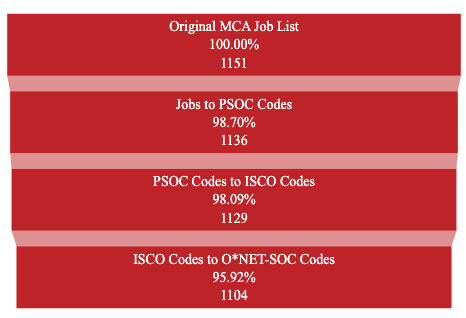
\includegraphics[width=0.8\linewidth]{../figures/funnel_jobs.png} 
    \caption{Funnel chart showing from MCA jobs to SOC codes.} 
    \label{fig:funnel_chart} 
\end{figure}

Because only a small amount of jobs were unmatched, ChatGPT was used to suggest suitable SOC codes. A full record of this process is available here: \href{https://chatgpt.com/share/68ca0dd0-46e0-8012-be0a-e825db6ec12f}{Job to SOC code mapping}.
Given now that each job in the MCA list has their corresponding SOC code, we can start determining their AIOE and complementarity scores.

